%%%%%%%%%%%%%%%%%%%%%%%%%%%%%%%%%%%%%%%%%%%%%%%%%%%%%%%%%%%%%%%%%%%%%%%%%%%%%%%%
\documentclass[twocolumn]{revtex4}
%\documentclass[12pt]{article}
%%%%%%%%%%%%%%%%%%%%%%%%%%%%%%%%%%%%%%%%%%%%%%%%%%%%%%%%%%%%%%%%%%%%%%%%%%%%%%%%
% Note that comments begin with a "%" and are not turned into text in the .pdf
% document.
%%%%%%%%%%%%%%%%%%%%%%%%%%%%%%%%%%%%%%%%%%%%%%%%%%%%%%%%%%%%%%%%%%%%%%%%%%%%%%%%

%%%%%%%%%%%%%%%%%%%%%%%%%%%%%%%%%%%%%%%%%%%%%%%%%%%%%%%%%%%%%%%%%%%%%%%%%%%%%%%%
% Include some extra packages.
%%%%%%%%%%%%%%%%%%%%%%%%%%%%%%%%%%%%%%%%%%%%%%%%%%%%%%%%%%%%%%%%%%%%%%%%%%%%%%%%
\usepackage[]{graphicx}
%%%%%%%%%%%%%%%%%%%%%%%%%%%%%%%%%%%%%%%%%%%%%%%%%%%%%%%%%%%%%%%%%%%%%%%%%%%%%%%%

%%%%%%%%%%%%%%%%%%%%%%%%%%%%%%%%%%%%%%%%%%%%%%%%%%%%%%%%%%%%%%%%%%%%%%%%%%%%%%%%
\begin{document}


%%%%%%%%%%%%%%%%%%%%%%%%%%%%%%%%%%%%%%%%%%%%%%%%%%%%%%%%%%%%%%%%%%%%%%%%%%%%%%%%
\title{
Will the person get away?
}

\author{Joseph Ferro }

\affiliation{Siena College, Loudonville, NY}

\date{\today}

\begin{abstract}
    Your abstract is a 1 paragraph summary of the project.
    You should summarize the motivation, the procedure, and the 
    results here.
    
    The purpose of this project is to find the probability of a human getting away from a velociraptor with a 30 meter head start. To solve for this probability I needed to first plot the speeds of the human and velociraptor on a position vs time graph. This showed where there speeds intersected but it did not show numbers. To see the time and distance that the velociraptor caught up with the human I wrote a function took the range of the two lines. Then had the function find where the two lines were equal and made it print. To find the time and distance for when the velociraptor attacked from one meter away I wrote a function. This was similar to the function for question two but this time I made a range that was in between 1 and 1.4. The last code is trying to find the probability that the person will be eaten or not. By using the Monte Carlo method and np.random.random I was able to figure out that there is about 60\% chance that the person will be eaten. The results state that a person will most likely not get away from a velociraptor even with a 30 meter head start. 
    
\end{abstract}

\maketitle
%%%%%%%%%%%%%%%%%%%%%%%%%%%%%%%%%%%%%%%%%%%%%%%%%%%%%%%%%%%%%%%%%%%%%%%%%%%%%%%%

%%%%%%%%%%%%%%%%%%%%%%%%%%%%%%%%%%%%%%%%%%%%%%%%%%%%%%%%%%%%%%%%%%%%%%%%%%%%%%%%
\section{Introduction}
%%%%%%%%%%%%%%%%%%%%%%%%%%%%%%%%%%%%%%%%%%%%%%%%%%%%%%%%%%%%%%%%%%%%%%%%%%%%%%%%

Before I began graphing I had to import

$$matplotlib.pylab as plt$$
$$ numpy as np$$

This pulls information from matplotlib to give me the ability to graph and Numpy is a Python  library that allows for complicated code.

$$t = np.linspace(0,20,10000)$$

Next I used $np.linspace$ to tell the computer to graph evenly 10000 data points between 1 and 20. The more points you ask the computer to graph the greater the accuracy. 

 
$$yh = 3*(t) + 30$$  
$$yr = 18*(t) + 0$$

The function $x_f = x_0 + v\Delta(t)$ was used to graph the data for both the velociraptor (yr) and the human (yh).

To actually plot the data I used the matplotlib.pylab as a plt. 

$$plt.plot(x,yh,'r-',linewidth=2,label='Human')$$
$$plt.plot(x,yr,'g-',linewidth=2,label='Veloceraptor')$$

The color of the lines of the graph was shown with $'r-'$ which means a red solid line. If it was $'r--'$ that would mean red dashed line. The velociraptor was $'g-'$ which means a green solid line. The last part is the $label =  'Human'$ and $label = 'Velociraptor'$ just names the lines in the legend. 

$$plt.xlabel('Time(s)',fontsize=18)$$
$$plt.ylabel('Position (m)',fontsize=18)$$

The $xlabel$ is the label for the x axis which I called Time(s) and $ylabel$ is the label for the y axis which I called Position(m).

$$plt.xlim(0,15)$$ 
$$plt.ylim(0,200)$$
This was used to set limits in the x and y axises on the graph so it is proportional. I made the limits to allow the reader to clearly see where the intersection of the two lines are. 

$$plt.title ("Will~he/she~ be~ Eaten")$$

plt.title labels the graph title.

$$plt.legend()$$

Legend allows the coder to name the lines.

\subsection{Question Two}

$$nyh = len(yh)$$
$$nyr = len(yr)$$

I made the new variables called nyh for the human and nyr for the velociraptor. The $len(yh)$ is a built in function that returns the length of yh and yr. Which is based off the $linspace$ in Question 1.

$$for~ i~ in~ range(nyh):$$

This is a range function that takes all the data nyh and takes the range of all of the data.


$$if yh[i] == yr[i]:$$

This is stating that when the lines intersect the function will stop. 

 $$print "Position ~of~ Human: \%f Position~ of ~Velociraptor$$
 $$:\%f Time: \%f" \% (yh[i], yr[i],t[i])$$

When the function stops its gonna print the position of the human, position of velociraptor and time. \%f is the format code for a float.

\subsection{ Question 3}
%%%%%%%%%% change
$$for i in range (nyr):$$

This generates a list of numbers from i which is then used to loop over in the range of  $len(yh)$. This was mentioned in question 2

$$if yh[i]-yr[i] <1:$$


In this if statement I subtracted human and the velociraptor and said it is less than 1. I did this because incase it wasn't exactly 1 alway the $$<1$$ says to the computer that it has to be close to 1. 

$$plt.plot([td,td],[0,200],..$$

This part is the magenta line that is parallel with the y axis. Since a line on a graph is essentially two points with a line connecting them, I decided to make a new variable td which was my new time. Then I just graphed the points (td,0) and (td,200) had them connected by a magenta line. 

\subsection{Question 4}

$$npts = 10000$$
$$t = np.random.random(1)$$

$np.random.random(1)$ returns random floats

$$for i in range (0,1000):$$

This functions loops through the range of 1000 data points 

$$ t = np.random.random(1)$$
$$if t[0]>.2:$$

This function is saying that if my t variable is greater then .2 then it will move onto the next function.

$$ t = np.random.random(1)$$
$$if t[0]>.15:$$

This function is saying that if my t variable is greater then .15 then it will move onto the next function. Since after every swipe the possibility of the velociraptor getting the human decreases. 

$$ t = np.random.random(1)$$
$$if t[0]>.07:$$

This function is saying that if my t variable is greater then .07 then the function stops because the velociraptor tries to get the human for only 3 swipes. 

$$p = (x/1000.0) * 100.0$$

This function is just the probability formula. The code puts in my x and divides it by 1000 because that is the amount of points of data that is there. Then it is multiplied by 100\% to make it a percentage. I had to make the numbers into decimals because this keeps it as a float. 

\section{Graphs and Calculations} 

\begin{figure}[h]
	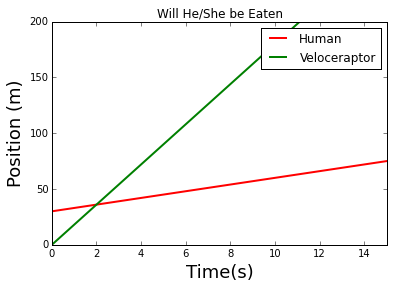
\includegraphics[width = 0.5\textwidth] {original_intersection.png}
	\caption{This is the position vs time graph of the both the velociraptor in green and the human in red. The velociraptor's line is steeper than the person because it moving at a velocity of 18m/s and the humans is 3 m/s. Since this graph represents velocity, the steeper the slope the greater the velocity. Where the lines intercept is when the velociraptor catches up to the human. The velocities were graph by using the formula $x_f= x_0 + v(t)$.This graphed the velocity of the graph. \label{fig:Graph when Velociraptor catches up to Person}}
\end{figure}

\begin{figure}[h]
	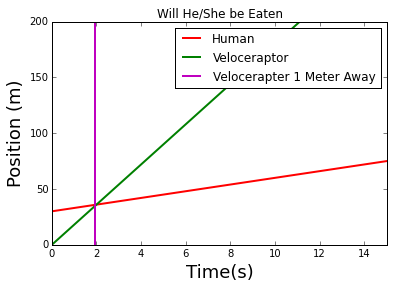
\includegraphics[width = 0.5\textwidth] {1_meter_away.png}
	\caption{This is the position vs time graph of both the velociraptor in green moving at 18 m/s  and the human in red, moving at 3 m/s. This graph shows when the velociraptor catches the human but also shows when the velociraptor is 1 meter away with a magenta line. The velocities were graph by using the formula $x_f = x_0 + v(t)$.   \label{fig:Graph when Velociraptor is 1 meter away from the Person}}
\end{figure}


\subsection{Finding the intersection of the graph for figure one}
$$x_f = x_0 + v\Delta(t) + \frac{1}{2}at$$
$$x_f =  v\Delta(t)$$
$$x_f = x_f$$
$$ x_0 + v_h\Delta(t)=  v_r\Delta(t)$$
$$\frac{x_0}{v_r - v_h} = t$$ 
$$ \frac{30m}{18- 3 }=t$$
$$ t = 2s$$

$$x_f = v \Delta(t)$$
$$x_f = 18 \frac{m}{s}(2s)$$
$$x_f = 36m$$



Explained:
The assumption was the human started running without acceleration and straight to top speed. Because of this assumption acceleration is 0 we were left with the second derivation. Setting these equal to each other found the time when they met and then plugging time back in gave the distance of 36 meters. This was plugged into the code and produced figure 1.

\subsection{Finding the intersection of graph for figure two when 1 meter away}
$$x_f = (x_0-1) + v\Delta(t) + \frac{1}{2}at$$
$$x_f = x_0 + v\Delta(t)$$
$$x_f = 30 + 3(t)$$

$$x_f = x_f$$
$$ x_0 + v_h\Delta(t)=  v_r\Delta(t)$$
$$\frac{x_0}{v_r - v_h} = t$$ 
$$ \frac{30m -1m}{18- 3 }=t$$
$$ t = 1.93s$$

$$x_r = v \Delta(t)$$
$$x_r = 18 \frac{m}{s}(1.93s)$$
$$x_r = 34.74m$$

$$x_h = x_0 + v\Delta(t)$$
$$x_h = 30m + 18\Delta(1.93)$$
$$x_h = 35.79m$$

Explained:
Similar to figure 1 I set both equations equal to each other and solved for time. However, since I'm solving for when the velociraptor is 1 meter away I subtracted 1 from the distance. This gave me the new time which was plugged into both equations because they are not at equal distances anymore. 
 \subsection{Probability} 

$$ p =  \frac{Number ~of~ favorable~ outcomes}{Total~ number ~of~ possible~ outcomes}$$

$$ p = \frac{x}{100000.0} 100.0$$

$$ p = 63\%$$

Explained:
Since I used $random.random$ the code will produce different percentages every time but all within the same range of 63\%. Probability tells how likely an event will happen. This is a prediction that the human will get away and with a 30 meter head start there is 63\% chance that the human will get away. 


\section{Results}

The purpose of this experiment was to find the probability of a human surviving an encounter with a velociraptor when the human has a 30 meter head start. Figure 1 shows when a velociraptor will catch up to the human but using the formula. $$x_f = x_0 + v(t)$$ The slope of the human is not as steep at the velociraptor because the human is running at only 3 m/s. The slope of the velociraptor is greater because it is moving at 18 m/s which is substantially greater. This is why the velociraptor is able to catch up to the human so quickly. To find the exact position and time the velociraptor meet I used the function$$for~ i~ in~ range(nyh):$$
$$if yh[i] == yr[i]:$$. This is telling the computer to loop through each point on the graph and find where the numbers equal. The computer said at 36 meters and in 2 seconds the velociraptor and the human will make contact.  Which by looking at the figure makes sense because it is under 40 on the y axis and at 2 seconds for the x axis. Figure 2 is the similar to Figure 1 because it used the same formula to graph the lines. However, Figure 2 has a magenta dot which is placed 1 meter away from the intersection. This is because the velociraptor will start attacking 1 meter away from the human. To solve for when the velociraptor is 1 meter I made a for loop in range which went through all of the data from $nyr = len(yr)$. Then by using an if statement I subtracted yh and yr and making a range between 1 and 1.4. This gave me the numbers for the velociraptor when it was 1 meter away. This states that the time for the velociraptor to reach the human at 1 meter away would be at 1.92 seconds. The last part of the experiment solved for the probability for the human to survive the attack. This was accomplished by a simple $$ t = np.random.random(1)$$ that plugged in 1000 random points into the function. Since the velociraptor would give up after three tries and the percentage for each attempt lessoned. I had to write three $$ t = np.random.random(1)$$ with decreasing percentages each time. At the end it was plugged into the a probability formula. $$ p = \frac{x}{100000.0} 100.0$$ The formula spit out percentages all between 63\%, meaning there was a 63\%  that the human would be eaten. Since I used numpy random it gave different percentages each time because it plugged in 100000 random numbers into the equation but they were all within 63\%. Originally I the only 1000 random numbers which gave me a greater range of percentages between 60\% and 64\%. By increasing the number of points that will be plugged increases the accuracy which I mentioned earlier. 





%%%%%%%%%%%%%%%%%%%%%%%%%%%%%%%%%%%%%%%%%%%%%%%%%%%%%%%%%%%%%%%%%%%%%%%%%%%%%%%%

%%%%%%%%%%%%%%%%%%%%%%%%%%%%%%%%%%%%%%%%%%%%%%%%%%%%%%%%%%%%%%%%%%%%%%%%%%%%%%%%

%%%%%%%%%%%%%%%%%%%%%%%%%%%%%%%%%%%%%%%%%%%%%%%%%%%%%%%%%%%%%%%%%%%%%%%%%%%%%%%%
\end{document}
%%%%%%%%%%%%%%%%%%%%%%%%%%%%%%%%%%%%%%%%%%%%%%%%%%%%%%%%%%%%%%%%%%%%%%%%%%%%%%%%
